\section{Web Server Module}

\subsection{APRS Middleware}
The APRS middleware will be responsible for processing the raw APRS data into a client compatible format.

\subsection{APRS Receiver}
The APRS receiver will be responsible for catching the raw APRS data sent by the APRS source.

\subsection{Client Transceiver}
The client transceiver will be responsible for receiving/sending data from/to all connected clients.

\subsection{Telemetry Middleware}
The telemetry middleware will be responsible for processing the raw telemetry data into a client compatible format.

\subsection{Telemetry Receiver}
The telemetry receiver will be responsible for catching the raw telemetry data sent by the telemetry source.

\subsection{Video Player}
The web server video player is rendered using the HTML5 defined video tag.

\subsection{Video Rendering}
The web server renders video through an open source javascript library. This library uses Media Source
Extensions (MSE), a W3C specification to provide browser support for Chromium and Firefox as well as the HTML5
video tag.

\begin{figure}[!ht]
  \centering
  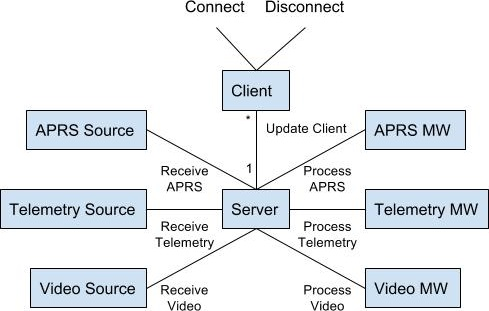
\includegraphics[scale=.8]{imgs/web_server.jpg}
  \caption{Web Server}
\end{figure}
